\chapter{Blockchain Essentials}
We cover the fundamentals needed to explain blockchain networks. At the first section, we start by covering fundamental cryptography concepts, next we cover the origin of blockchains; Bitcoin and how it works, then we continue with Ethereum and how it expanded and diverged from Bitcoin.
% and finally we abstract and summarize the attributes of blockchains.

\section{General Background}
This section covers basic cryptographic concepts that run the web of trust today.

\subsection{Cryptographic Hash Functions}
A cryptographic hash function is a computationally efficient mathematical algorithm, that has certain properties which make it suitable for cryptography. It maps data of arbitrary size to a bit string of fixed size, known as hash. The slightest change to the input makes a large change in the resulting hash. Designed to be a one-way function, it is easy to produce the output given the input but computationally infeasible to produce the input given the output. In theoretical cryptography, the security level of a cryptographic hash function has been defined using the following properties. \footnote{$H$ is a hash function with inputs $x,x'$ and outputs $y,y'$} \cite{katz1996handbook}

\begin{enumerate} 
    \item \textbf{Preimage resistance}: It is computationally infeasible to find any input $x$ which hashes to that output $y$. Given $y$, it is difficult to find any preimage $x'$ such that $H(x')=y$ when given any $y$ for which the corresponding input $x$ is not known. 
    \item \textbf{Second preimage resistance}: It is computationally infeasible to find any second input which has the same output as any specified input, that is given $x$ to find a 2nd-preimage $x'\neq x$ such that $H(x)=H(x')$.
    \item \textbf{Collision Resistance}: It is computationally infeasible to find any two distinct inputs $x,x'$ which hash to the same output such that $H(x)=H(x')$
\end{enumerate}
\subsection{Public Key Cryptography}
\acrfull{pki} also referred to as asymmetric cryptography, is a system that uses a pair of keys, a \textit{public key} $e$ that is widely known and a corresponding \textit{private key} $d$ which is known only to the owner. The two keys have a mathematical relationship and in secure systems the task of computing $d$ given $e$ is computationally infeasible. In such a system, any person can encrypt a message using the receiver's \textit{public key} and that encrypted message can only be decrypted by the receiver's \textit{private key}. The public key defines an \textit{encryption transformation} $E_e$, while the private key defines the associated \textit{decryption transformation} $D_d$. Any entity $B$ wishing to send a message $m$ to $A$ obtains $A$'s public key $e$, uses the encryption transformation to obtain the \textit{ciphertext} $c=E_e(m)$ and transmits $c$ to $A$. To decrypt $c$, $A$ applies the decryption transformation to obtain the original message $m=D_d(c)$

% How do we achieve integrity and non repudiation with public key cryptography?
Public key cryptography establishes a secure communication by satisfying the following cryptographic objectives:
\begin{enumerate}
    \item \textbf{Confidentiality}: Keeps the content of information from all but those authorized to have it. Achieved by encrypting, $B$ uses $A$'s public key to encrypt the message and only $B$ can decrypt that message with its private key, but anyone could impersonate $A$.
    \item \textbf{Data Integrity}: Addresses the unauthorized alteration of data using digital signatures. Digital signatures is a scheme where both parties verify that the information sent was created by the claimed sender and has not been tampered with. Entity $A$ uses its private key to produce a hash of the message and attaches it as a signature to the message. Entity $B$ receives the signed message and uses the same hash algorithm that $A$ used with its public key. Finally it compares the resulting hash with the message's actual hash, if the two are equal then it knows the author is the one with the possession of the particular private key.
    \item \textbf{Authentication}: Associated with identification and applied to both entities and the data itself, which implicitly provides data integrity. Achieved by encrypting ones message with its own private key, $B$ uses its private key to encrypt the message and send it to $A$, it can decrypt the message using $B$'s public key and thus verifying the sender, but anyone intercepting the communication can decrypt it.
    \item \textbf{Non-repudiation} Prevents an entity from denying actions by using digital signatures, a procedure that involves a trusted third party to resolve the dispute. i.e  $A$ authorizes a transaction to sent an asset to $B$ and later denies it. Since the transaction is signed with $A$'s private key, there is no room questioning.
\end{enumerate}
\begin{figure}[H]
        \centering
        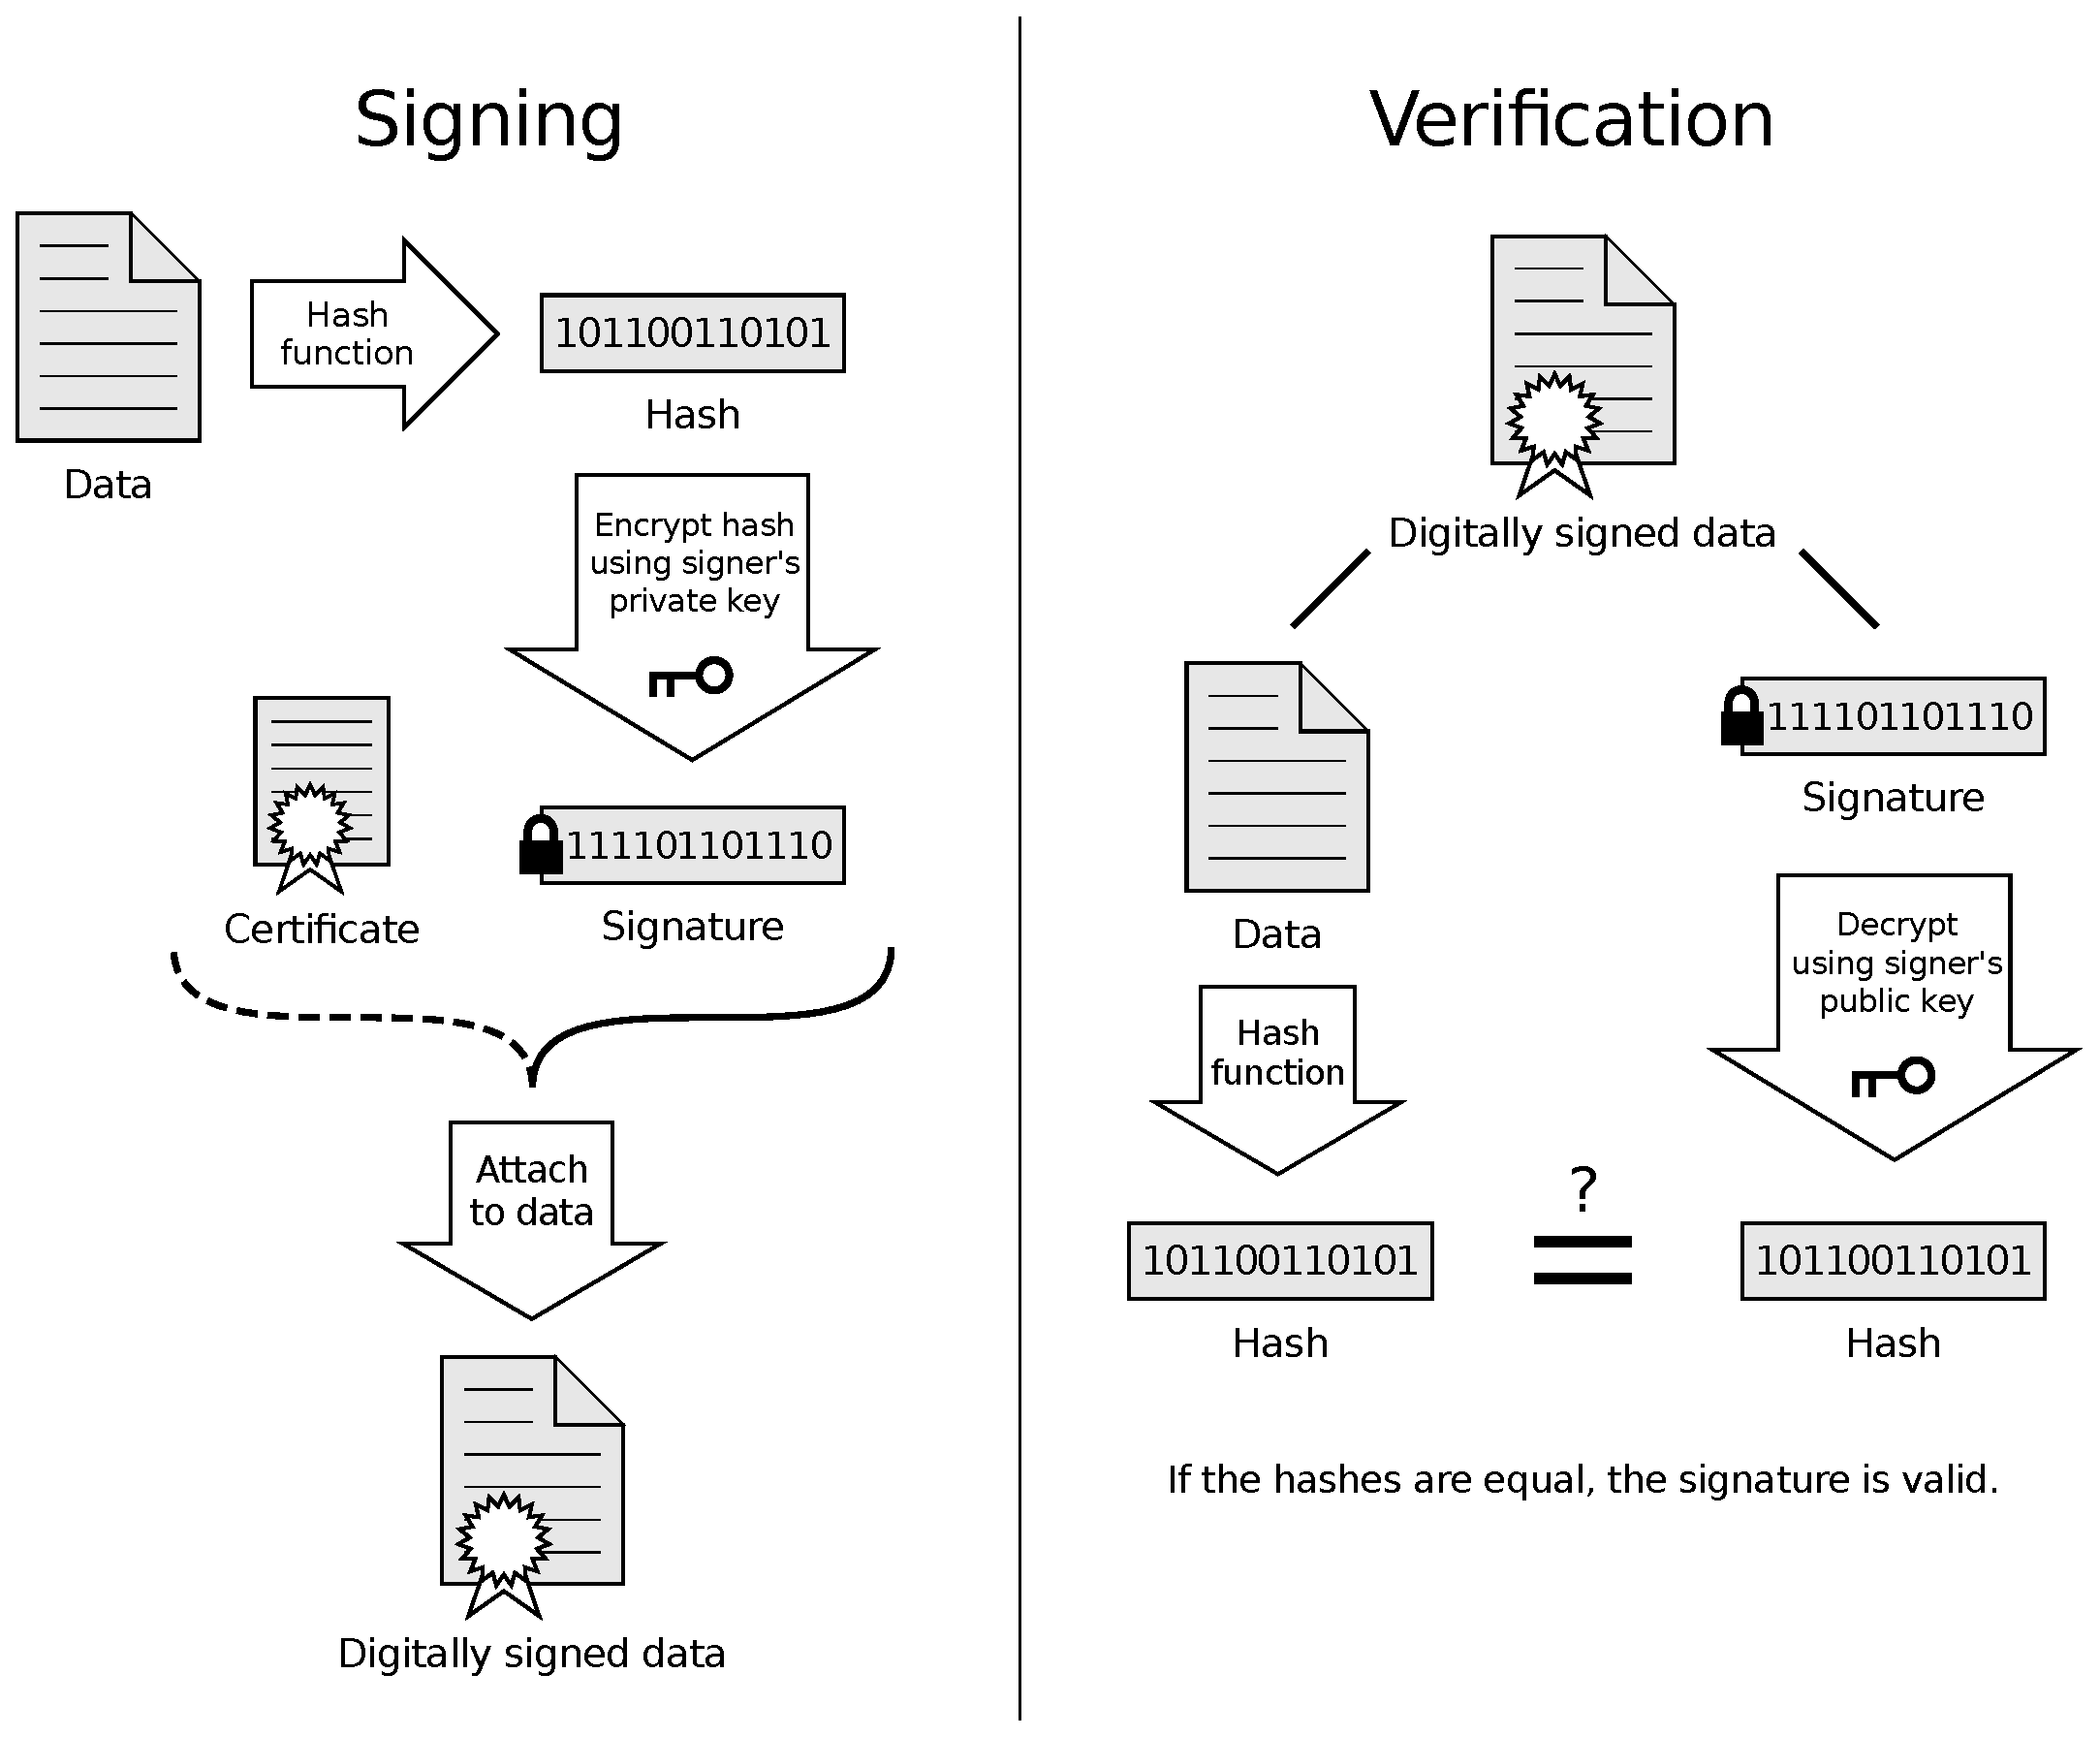
\includegraphics[width=1\textwidth]{Digital_Signature_diagram.eps}
        \caption{How digital signing works \cite{wiki:digital-signature}.}
        \label{fig:dig_sign}
    \end{figure}	
\subsection{Public Key Infrastructure}
In this subsection we cover the basics of Public Key infrastructure in order to associate them later to Fabric's components. 
PKI comprises \cite{CertificatesPKI} :
\begin{itemize}
    \item \textbf{\acrfull{ca}}: A trusted node that acts as a maintainer, keeping the public keys for all nodes. The \acrshort{ca} also bootstraps newly joined nodes in the network by adding their public key to their list, thus only the new node and the \acrshort{ca} need to be configured. 
    \item \textbf{Certificates}: A signed document, as a passport, issued by the \acrshort{ca} stating that a particular name holds a particular private key. Other parties, knowing the public key of \acrshort{ca}, can authenticate a user.  
    \item A repository for retrieving certificates.
    \item A method of revoking certificates.
    \item A method of evaluating a chain of certificates from known public keys to the target name.
\end{itemize}